\begin{minipage}{0.75\linewidth}
\begin{figure}[h]
    \centering
    \begin{adjustbox}{max width=1.0\linewidth, keepaspectratio}
        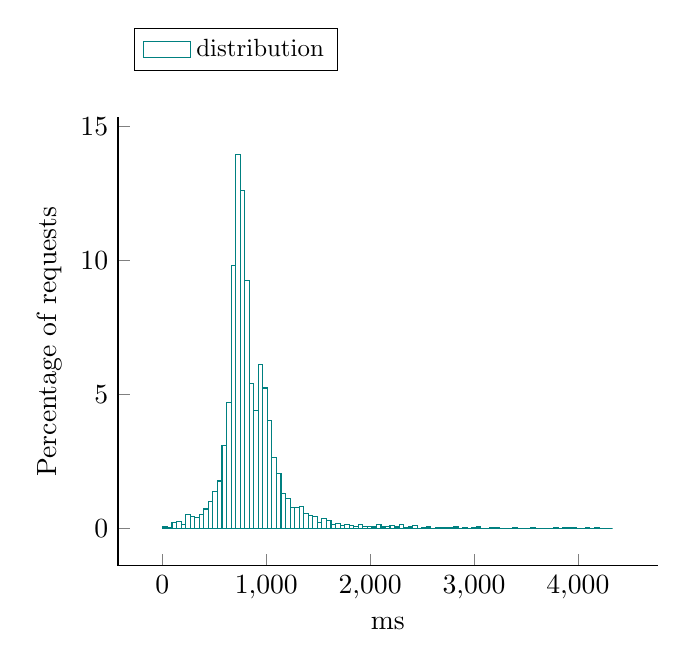
\begin{tikzpicture}
            \begin{axis}[ylabel = Percentage of requests, 
xlabel = ms, 
legend style = {nodes={scale=0.9, transform shape}, at={(0.03,1.2)}, anchor=north west, draw=black, fill=white, align=left, legend columns=3},
area style, mark size = 0pt,
 cycle list name = exotic,
  axis lines* = left]
		\addplot +[ybar interval] coordinates {
			 (5, 0.046875)
			 (48.73, 0.015625)
			 (92.46, 0.203125)
			 (136.19, 0.265625)
			 (179.92, 0.15625)
			 (223.65, 0.53125)
			 (267.38, 0.4375)
			 (311.11, 0.40625)
			 (354.84, 0.515625)
			 (398.57, 0.71875)
			 (442.3, 0.984375)
			 (486.03, 1.35938)
			 (529.76, 1.76562)
			 (573.49, 3.07812)
			 (617.22, 4.6875)
			 (660.95, 9.8125)
			 (704.68, 13.9375)
			 (748.41, 12.5938)
			 (792.14, 9.23438)
			 (835.87, 5.39062)
			 (879.6, 4.40625)
			 (923.33, 6.125)
			 (967.06, 5.23438)
			 (1010.79, 4.03125)
			 (1054.52, 2.625)
			 (1098.25, 2.03125)
			 (1141.98, 1.29688)
			 (1185.71, 1.125)
			 (1229.44, 0.765625)
			 (1273.17, 0.765625)
			 (1316.9, 0.796875)
			 (1360.63, 0.546875)
			 (1404.36, 0.484375)
			 (1448.09, 0.4375)
			 (1491.82, 0.21875)
			 (1535.55, 0.375)
			 (1579.28, 0.28125)
			 (1623.01, 0.15625)
			 (1666.74, 0.1875)
			 (1710.47, 0.09375)
			 (1754.2, 0.140625)
			 (1797.93, 0.09375)
			 (1841.66, 0.078125)
			 (1885.39, 0.140625)
			 (1929.12, 0.0625)
			 (1972.85, 0.078125)
			 (2016.58, 0.046875)
			 (2060.31, 0.125)
			 (2104.04, 0.046875)
			 (2147.77, 0.0625)
			 (2191.5, 0.109375)
			 (2235.23, 0.046875)
			 (2278.96, 0.140625)
			 (2322.69, 0.03125)
			 (2366.42, 0.046875)
			 (2410.15, 0.109375)
			 (2453.88, 0)
			 (2497.61, 0.03125)
			 (2541.34, 0.046875)
			 (2585.07, 0)
			 (2628.8, 0.015625)
			 (2672.53, 0.015625)
			 (2716.26, 0.015625)
			 (2759.99, 0.015625)
			 (2803.72, 0.046875)
			 (2847.45, 0)
			 (2891.18, 0.03125)
			 (2934.91, 0)
			 (2978.64, 0.015625)
			 (3022.37, 0.046875)
			 (3066.1, 0)
			 (3109.83, 0)
			 (3153.56, 0.03125)
			 (3197.29, 0.03125)
			 (3241.02, 0)
			 (3284.75, 0)
			 (3328.48, 0)
			 (3372.21, 0.015625)
			 (3415.94, 0)
			 (3459.67, 0)
			 (3503.4, 0)
			 (3547.13, 0.015625)
			 (3590.86, 0)
			 (3634.59, 0)
			 (3678.32, 0)
			 (3722.05, 0)
			 (3765.78, 0.015625)
			 (3809.51, 0)
			 (3853.24, 0.015625)
			 (3896.97, 0.015625)
			 (3940.7, 0.03125)
			 (3984.43, 0)
			 (4028.16, 0)
			 (4071.89, 0.015625)
			 (4115.62, 0)
			 (4159.35, 0.03125)
			 (4203.08, 0)
			 (4246.81, 0)
			 (4290.54, 0)
			 (4334.27, 0)
		};
\addlegendentry{distribution};
           \end{axis}
      \end{tikzpicture}
  \end{adjustbox}
  \caption{Response time distribution - req = ReadTimeline-2}
\end{figure}
\end{minipage}\hfill\begin{minipage}{0.18\linewidth}
\begin{table}[h]
\begin{tabular}{|cc|}
\hline
\textbf{} & \textbf{ms}\\ \hline
 \Xhline{0.005\arrayrulewidth}
min & 5\\
 \Xhline{0.005\arrayrulewidth}
max & 4378\\
 \Xhline{0.005\arrayrulewidth}
mean & 853\\
 \Xhline{0.005\arrayrulewidth}
std & 319\\
\hline
\hline
 \Xhline{0.005\arrayrulewidth}
25th & 705\\
 \Xhline{0.005\arrayrulewidth}
50th & 786\\
 \Xhline{0.005\arrayrulewidth}
75th & 956\\
 \Xhline{0.005\arrayrulewidth}
80th & 991\\
 \Xhline{0.005\arrayrulewidth}
85th & 1043\\
 \Xhline{0.005\arrayrulewidth}
90th & 1126\\
 \Xhline{0.005\arrayrulewidth}
95th & 1346\\
 \Xhline{0.005\arrayrulewidth}
99th & 2202\\
\hline
\end{tabular}
\caption{Response time}
\end{table}
\end{minipage}\hfill